% Prof. Dr. Ausberto S. Castro Vera
% UENF - CCT - LCMAT - Curso de Ci\^{e}ncia da Computa\c{c}\~{a}o
% Campos, RJ,  2019
% Disciplina: An\'{a}lise e Projeto de Sistemas
% Aluno:

\chapterimage{projeto.png} % Table of contents heading image
\chapter{Projeto do Sistema}
 Neste capítulo será apresentado as estratégias de implementação  do sistema.

\section{Estrat\'{e}gia do Projeto}

A secção a seguir serão apresentados os tipos de estratégias para construção do projeto.

    \subsection{Personalizado}
    O Projeto é criado de forma exclusiva para empresa, com intuito de atender as suas necessidades. É um modelo recomendado para grandes projetos , devido a quantidades de requisitos e as exigências que o sistema requer, impossibilitando que seja encontrado soluções prontas para atender os requisitos.

 É um sistema que permite aos desenvolvedores maior liberdade na solução de problemas do negócio.

O sistema hospitalar será construído baseado no modelo de sistema personalizado, devido a grande quantidade de requisitos e a complexidade do sistema.



    \subsection{Software Pronto}
    É o sistema que atende todos requisitos é comprado pela empresa já pronto,  onde não é necessário modificar os requisitos do sistema. Esse modelo é recomendado para empresas que não tenha necessidades de negócios exclusivo pequenas.  Ex: Sistema de caixa de supermercado e controle de estoque de farmácia.

    \subsection{Terceirização}
    
    O sistema é feito por uma outra  empresa especializada na construção de sistemas. Esse modelo é arriscado, devido a empresa contratada necessitar ter o total conhecimentos dos requisitos e a necessidade de negócios da empresa contratante.





\section{Arquitetura do Sistema - Estilos}
A secção a seguir sera apresentado 3 tipos de arquitetura de sistema.

    \subsection{Arquitetura do Hardware}
         \begin{itemize}
    \item \textbf{Internet}
  \end{itemize}
\begin{figure}[H]
              \begin{center}
                  \caption{Diagrama de internet do tipo pipe} \label{afp}
                  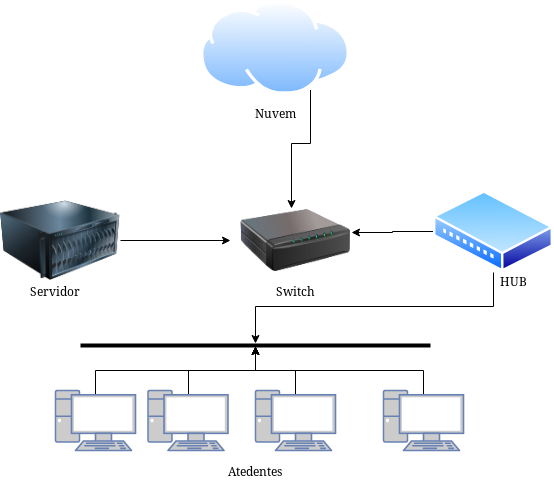
\includegraphics[width=15cm]{Pictures/DiagramaDeInternetTipoPipe.png} \\

              \end{center}
             \end{figure}
             
             
         \begin{itemize}
         
    \item \textbf{Servidor}
  \end{itemize}
\begin{figure}[H]
              \begin{center}
                  \caption{Diagrama de internet do tipo pipe} \label{afp}
                  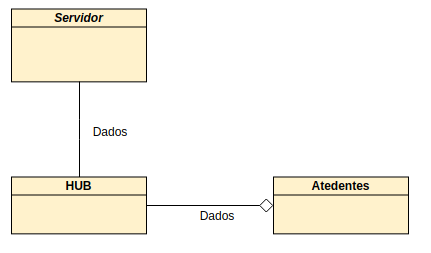
\includegraphics[width=15cm]{Pictures/DiagramaDeServidorTipoObjeto.png} \\

              \end{center}
             \end{figure}



    \subsection{Arquitetura do Sistema}
    
    \begin{itemize}
    
    \item \textbf{Medicamentos}
  \end{itemize}
\begin{figure}[H]
              \begin{center}
                  \caption{Diagrama de Medicamentos tipo objeto} \label{afp}
                  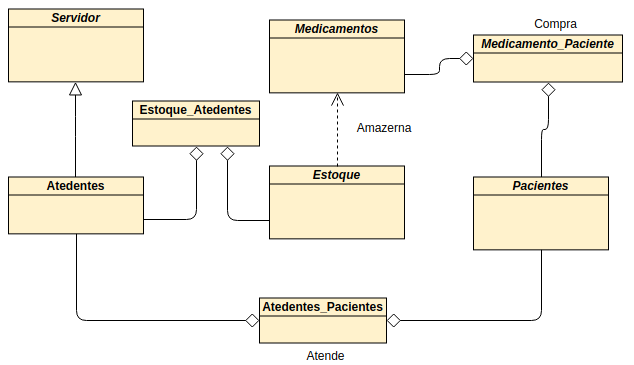
\includegraphics[width=15cm]{Pictures/DiagramaMedicamentoTipoObjeto.png} \\

              \end{center}
             \end{figure}
             
             \begin{itemize}
             
    \item \textbf{Atendimento}
  \end{itemize}
\begin{figure}[H]
              \begin{center}
                  \caption{Diagrama de atendimento tipo servidor} \label{afp}
                  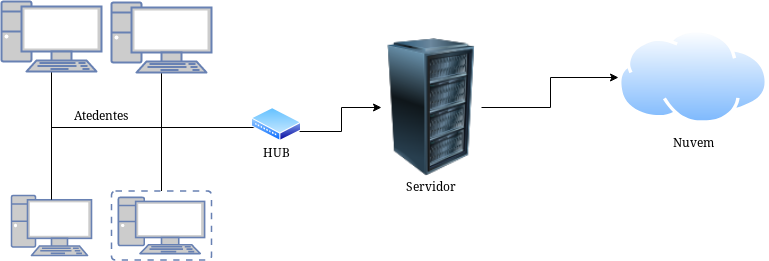
\includegraphics[width=15cm]{Pictures/DiagramaAtendimentoTipoServidor.png} \\

              \end{center}
             \end{figure}




    \subsection{Arquitetura de Software}
    

 \begin{itemize}
 
    \item \textbf{Atendimento}
  \end{itemize}
\begin{figure}[H]
              \begin{center}
                  \caption{Diagrama de atendimento tipo objeto} \label{afp}
                  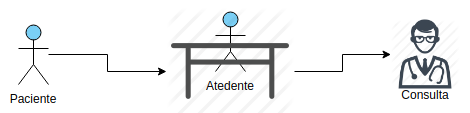
\includegraphics[width=15cm]{Pictures/DiagramaAtendimentoTipoObjeto.png} \\

              \end{center}
             \end{figure}

